\subsection{Fire brigade}
\label{sec:firefighters}
Similarly to the ambulance team and police force, fire brigade agents will be divided in sectors of the map. %The number of sectors depends on map size and number of fire brigades. % on the whole map. 
A score will be assigned to each sector, depending on its importance. For the fire brigades, the importance of a sector depends on the number of burning buildings and the disaster potential of the sector. The disaster potential is related to buried civilians, gas stations and building density of a sector. Building density takes into account the total area (ground area $\times$ number of floors) of all buildings in a sector. We want to prevent fire from spreading to buildings with buried civilians, to gas stations and to areas with high building density.

Firefighters will assign a score to each burning building depending on the ``effort'' needed to extinguish the fire on the building. The effort is related to the amount of water and time required to control the fire on a building. To calculate the effort, we need a model of how fire evolves in a building along time. This model will be given by a regression over the attributes of the building that the fire brigade agent can observe: fieryness, temperature, material and total area.

Data for the regression is extracted from the simulator logs. After several runs on different maps, a significant amount of data from different buildings can be obtained and used as input for the regression.

\subsubsection{Task Allocation}

Firefighters assign a score to each building. The score takes into account the importance of the building (the ones with buried civilians and/or located near gas stations are more important), the agent-to-building distance and effort needed to extinguish the fire. Effort estimation takes as input the prediction of how fire evolves (obtained from the regression model previously discussed) and returns a measure of water and time needed to control the fire. The importance of the building increases its score whereas the distance and the effort decreases its score (a fire brigade agent will prefer to extinguish fires on close, important buildings that do not require too much effort). Figure \ref{fig:firebrigade} shows how a firefighter calculates the score of a building.

\begin{figure}[!ht]
     \centering
     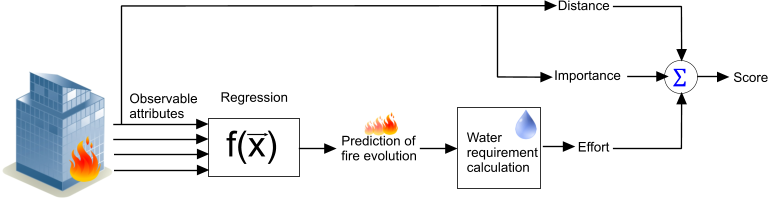
\includegraphics[width=12cm]{img/firebrigade.png}
     \caption{Building score calculation procedure performed by fire brigade agents.}
     \label{fig:firebrigade}
\end{figure}


After deciding which fire to fight, the firefighter calculates whether it is able to extinguish the fire alone. If not, the agent requests help from teammates, using the recruitment method discussed in Section \ref{sec:recruiting}.
